\subsection{Day 2} \label{sec:day2}

The daily meeting took place as planned at 11:00 PST. \footnote{\url{https://confluence.lsstcorp.org/display/DM/OPS+Rehearsal+\%28Day+2\%3A+2020-07-29\%29+Meeting+notes}}

Initial data tests took O(2 hours).  Second test provided calibrations for the
second night (flats should not show condensation).

Transfers again slow and DB access not provided in monitoring scripts so
relying on file creation times (fixes were added after the meeting).  LHN
persons are looking at slow transfer speeds.

Processing proceeded similar to the night before.  Provisional changes in
CALIB area permissions worked but still unclear how to see logs.  One dark frame
had problems with only 6 of 9 files being transferred (required a restart).

Quality analyses showed a huge change in flat frames (confirming that
moisture indeed impacted previous calibrations).


\begin{figure}
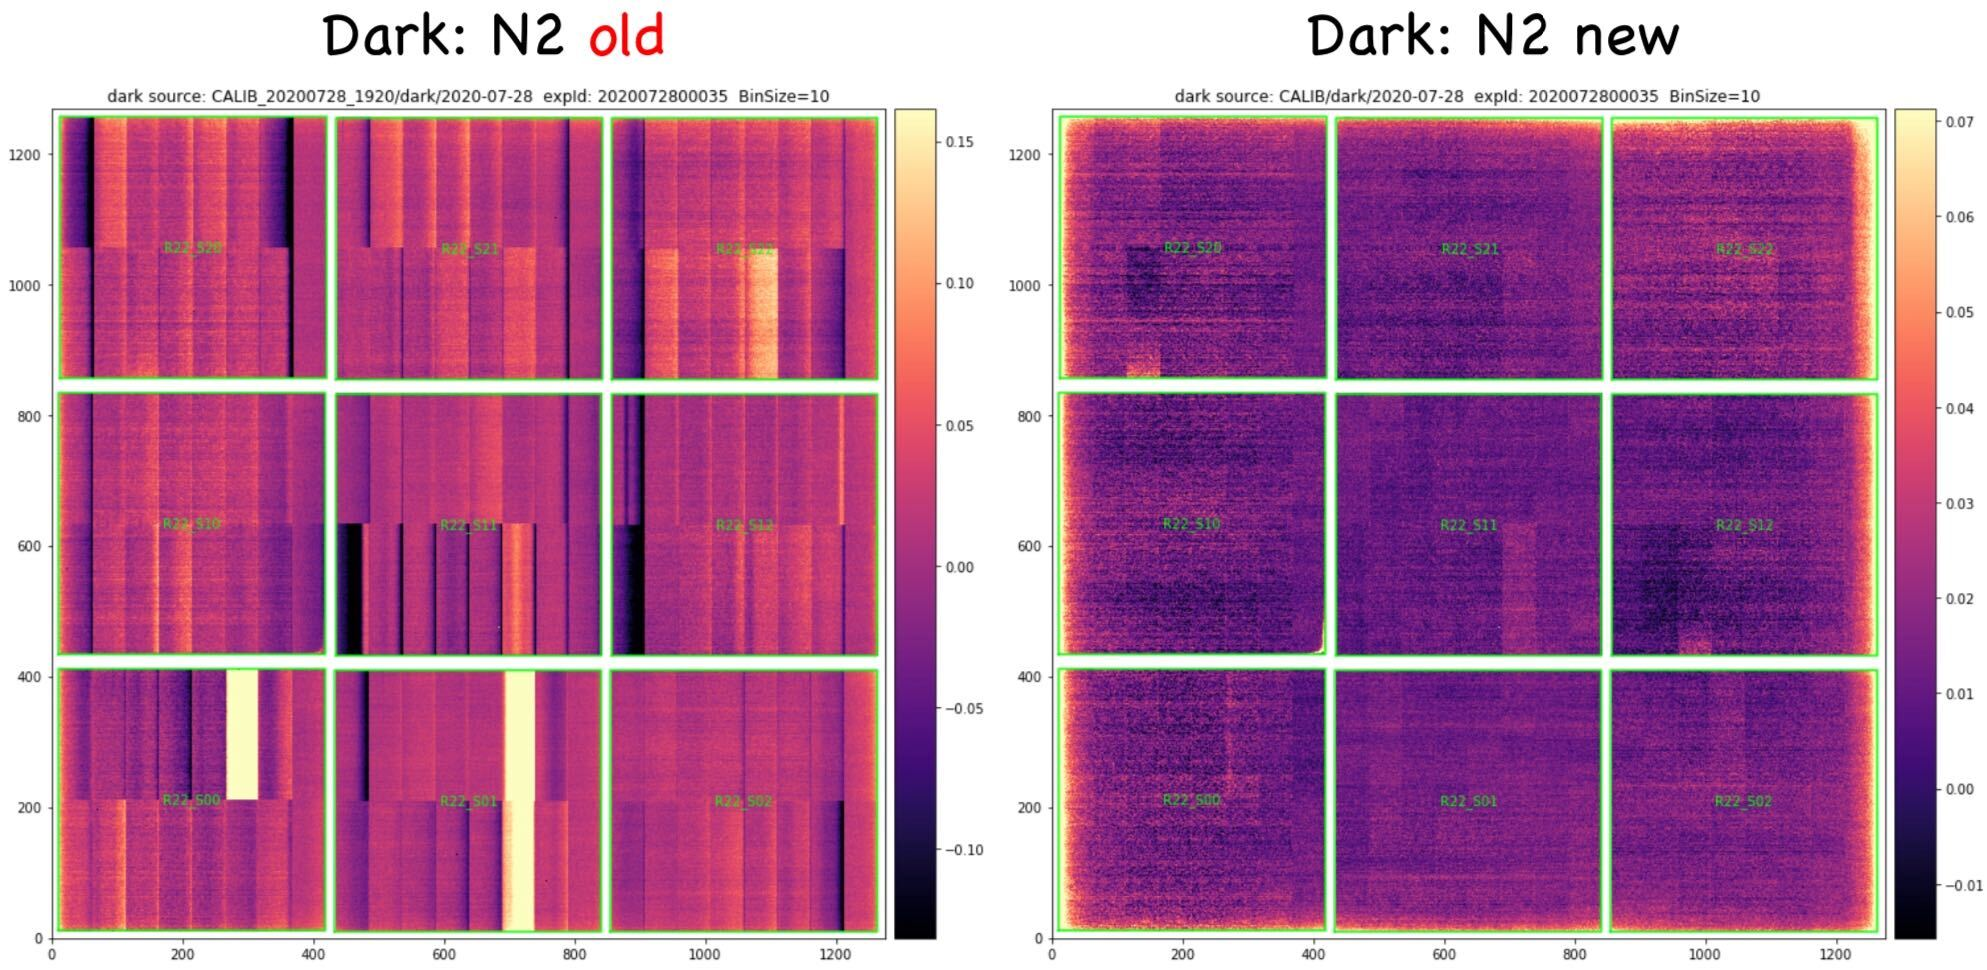
\includegraphics[width=0.6\textwidth]{figures/n2bad}
\caption{Night two flat still with incorrect bias subtraction.\label{fig:d2}}
\end{figure}

\subsubsection{Discussion}

The plans for the next night were discussed.  Initially there were supposed to be
changes, with an aborted flat sequence followed by change in illumination prior to
the "real" sequence being taken.  This plan was altered in favor of attempting to
get some preliminary estimates about the overall stability of the instrument from
one night to the next while in its temporary (not so stable) environment.  So the
upcoming calibration sequences were planned to have no explicit changes.


